\documentclass[11pt,a5paper]{article}

\usepackage[T1]{fontenc}
\usepackage[utf8]{inputenc}
\usepackage{lmodern, microtype}
\usepackage[estonian]{babel}
\usepackage{siunitx}
\sisetup{inter-unit-product=\ensuremath{{\cdot}}, per-mode=fraction, exponent-product=\cdot, output-decimal-marker={,}}
\usepackage{graphicx}
\usepackage{wrapfig}
\usepackage{adjustbox}
\usepackage{amsmath,amssymb}
\usepackage{amsfonts}
\usepackage[hidelinks]{hyperref}
\usepackage{csquotes}
\usepackage{caption}
\usepackage{enumitem}
\usepackage{soulutf8}
\usepackage[all]{nowidow}
\topmargin=-3.0cm \textheight=19cm \textwidth=12.9cm
\oddsidemargin=-1.5cm  \evensidemargin=-1.5cm
\setlength{\parindent}{0pt} \setlength{\parskip}{6pt} \sloppy
\sloppy \relpenalty=10000 \binoppenalty=10000
\pagestyle{empty}

\newcommand{\numb}[1]{\vspace{5pt}\textbf{\large #1}}
\newcommand{\nimi}[1]{(\textsl{\small #1})}
\newcommand{\punktid}[1]{(\emph{#1~p.})}
\newcommand{\p}[1]{[\textbf{#1~p}]}
\newcounter{ylesanne}
\newcounter{expylesanne}
\newcommand{\yl}[1]{\addtocounter{ylesanne}{1}\numb{\theylesanne.} \nimi{#1} \newblock{}}
\newcommand{\expyl}[1]{\addtocounter{expylesanne}{1}\numb{E\theexpylesanne.} \nimi{#1} \newblock{}}
%\newcommand{\autor}[1]{}% Kasuta võistluse ajal
\newcommand{\autor}[1]{\emph{Autor: #1}}% Kasuta kui vaja autorit
\renewcommand{\leq}{\leqslant}
\renewcommand{\geq}{\geqslant}

\newenvironment{skeemlist}{\begin{itemize}[nosep, topsep=0pt, leftmargin=*]}{\end{itemize}}
\newenvironment{skeem}{\emph{Hindamisskeem}:\begin{skeemlist}}{\end{skeemlist}}

\begin{document}
\normalsize
\begin{center}
  \textbf{\Large Eesti koolinoorte 71.\ füüsikaolümpiaad} \par
  \emph{9.\ veebruar 2024. a. Piirkondlik voor.\\ Gümnaasiumi ülesannete lahendused (10.--12.\ klass).}
\end{center}

\normalsize

\numb{Eessõna}

Allpool on toodud iga ülesande üks õige lahenduskäik (mõnel juhul ka enam). \textbf{Kõik alternatiivsed õiged lahenduskäigud tuleb hinnata samuti maksimumpunktidega.} Iga alternatiivse lahenduskäigu jaoks tuleb kontrollijatel koostada hindamisskeem, juhindudes võimalusel juuresoleva hindamisskeemi punktijagamisproportsioonist. Soovituslikud mahaarvamise punktid:
\begin{skeemlist}
  \item numbriline arvutusviga --- \p{0,5};
  \item viga teisendustes --- \p{0,5} (märgi jms väiksem viga) või \p{1} (viga, mis viib dimensioonide konfliktini), maha arvata ainult üks kord, st edasikanduvat viga mitte karistada;
  \item kui vastus tuleb füüsikaliselt absurdne, siis võib täiendavalt karistada \p{0,5};
  \item üksik viga lähtevalemis --- \p{0,5} (kui märgiviga) kuni \textbf{50\%} (sisuline viga).
\end{skeemlist}
\vspace{1em}

\yl{PÄIKESEPANEEL}
\punktid{6} \autor{Richard Luhtaru}

Iga paneeli poolt toodetav keskmine energia võimsus on
\begin{equation*}
    P = \eta S I = \SI{24.75}{\W}. \quad\p{2}
\end{equation*}

Pille keskmine energiatarbimise võimsus on
\begin{equation*}
    P_k = \frac{\SI{3000}{\kWh}}{\SI{1}{aasta}} \cdot \frac{\SI{1000}{W}}{\SI{1}{kW}}\cdot\frac{\SI{1}{aasta}}{\num{365}\cdot\SI{24}{h}} \approx \SI{342.5}{W}. \quad\p{2}
\end{equation*}

Leiame, et
\begin{equation*}
    \frac{P_k}{P} = \frac{\SI{342.5}{W}}{\SI{24.75}{W}} \approx \num{13.8}, \quad\p{1}
\end{equation*}
seega Pillel on vaja vähemalt 14 päikesepaneeli. \p{1}

\yl{HAJUMINE}
\punktid{6} \autor{Moorits Mihkel Muru}

Tajur mõõdab valgustihedust ehk valgustatust, seega mida suurema ala peale valgusallikast pärinev valgus hajub, seda väiksem on tajuri näit. Olgu valgusallika võimsus $P$ ja valgusallikast tuleva valgusvihu pindala $S_1$, siis esimeses katses mõõdetud tajuri näitu kirjeldab suurus $E_1 = P/S_1 = P/\pi r_1^2$, kui eeldada, et valgusvihu pindala on ringikujuline ja raadiusega $r_1$. Teises katses kirjeldab tajuri väärtust suurus $E_2 = P/S_2 = P/\pi r_2^2$, kus $r_2$ sõltub sellest, kui kaugel tajur peeglist on. Raadiuse $r_2$ saab avaldada läbi raadiuse $r_1$ kasutades teadmist, et kumerpeeglile lastud paralleelne kiirtekimp koondub fookuses, mis asub kumerpeegli pinnast kaugusel $R/2$. Tekivad sarnased kolmnurgad, millest esimese kõrgus on $R/2$ ja alus $2r_1$ ning teise kõrgus on $R/2 + L$ ning alus $2r_2$. Seega saame
$$ \frac{R/2}{2r_1} = \frac{R/2 + L}{2r_2} \Rightarrow r_2 = \frac{R/2 + L}{R/2} r_1$$
ja tajuri näitude suhe on
$$ \frac{E_1}{E_2} = \frac{P/S_1}{P/S_2} = \frac{S_2}{S_1} = \frac{r_2^2}{r_1^2} = \left(\frac{R/2 + L}{R/2}\right)^2 = \left(\frac{\SI{15}{\centi\meter} + \SI{60}{\centi\meter}}{\SI{15}{\centi\meter}}\right)^2 = 25 \ .$$

\begin{figure}[h]
    \centering
    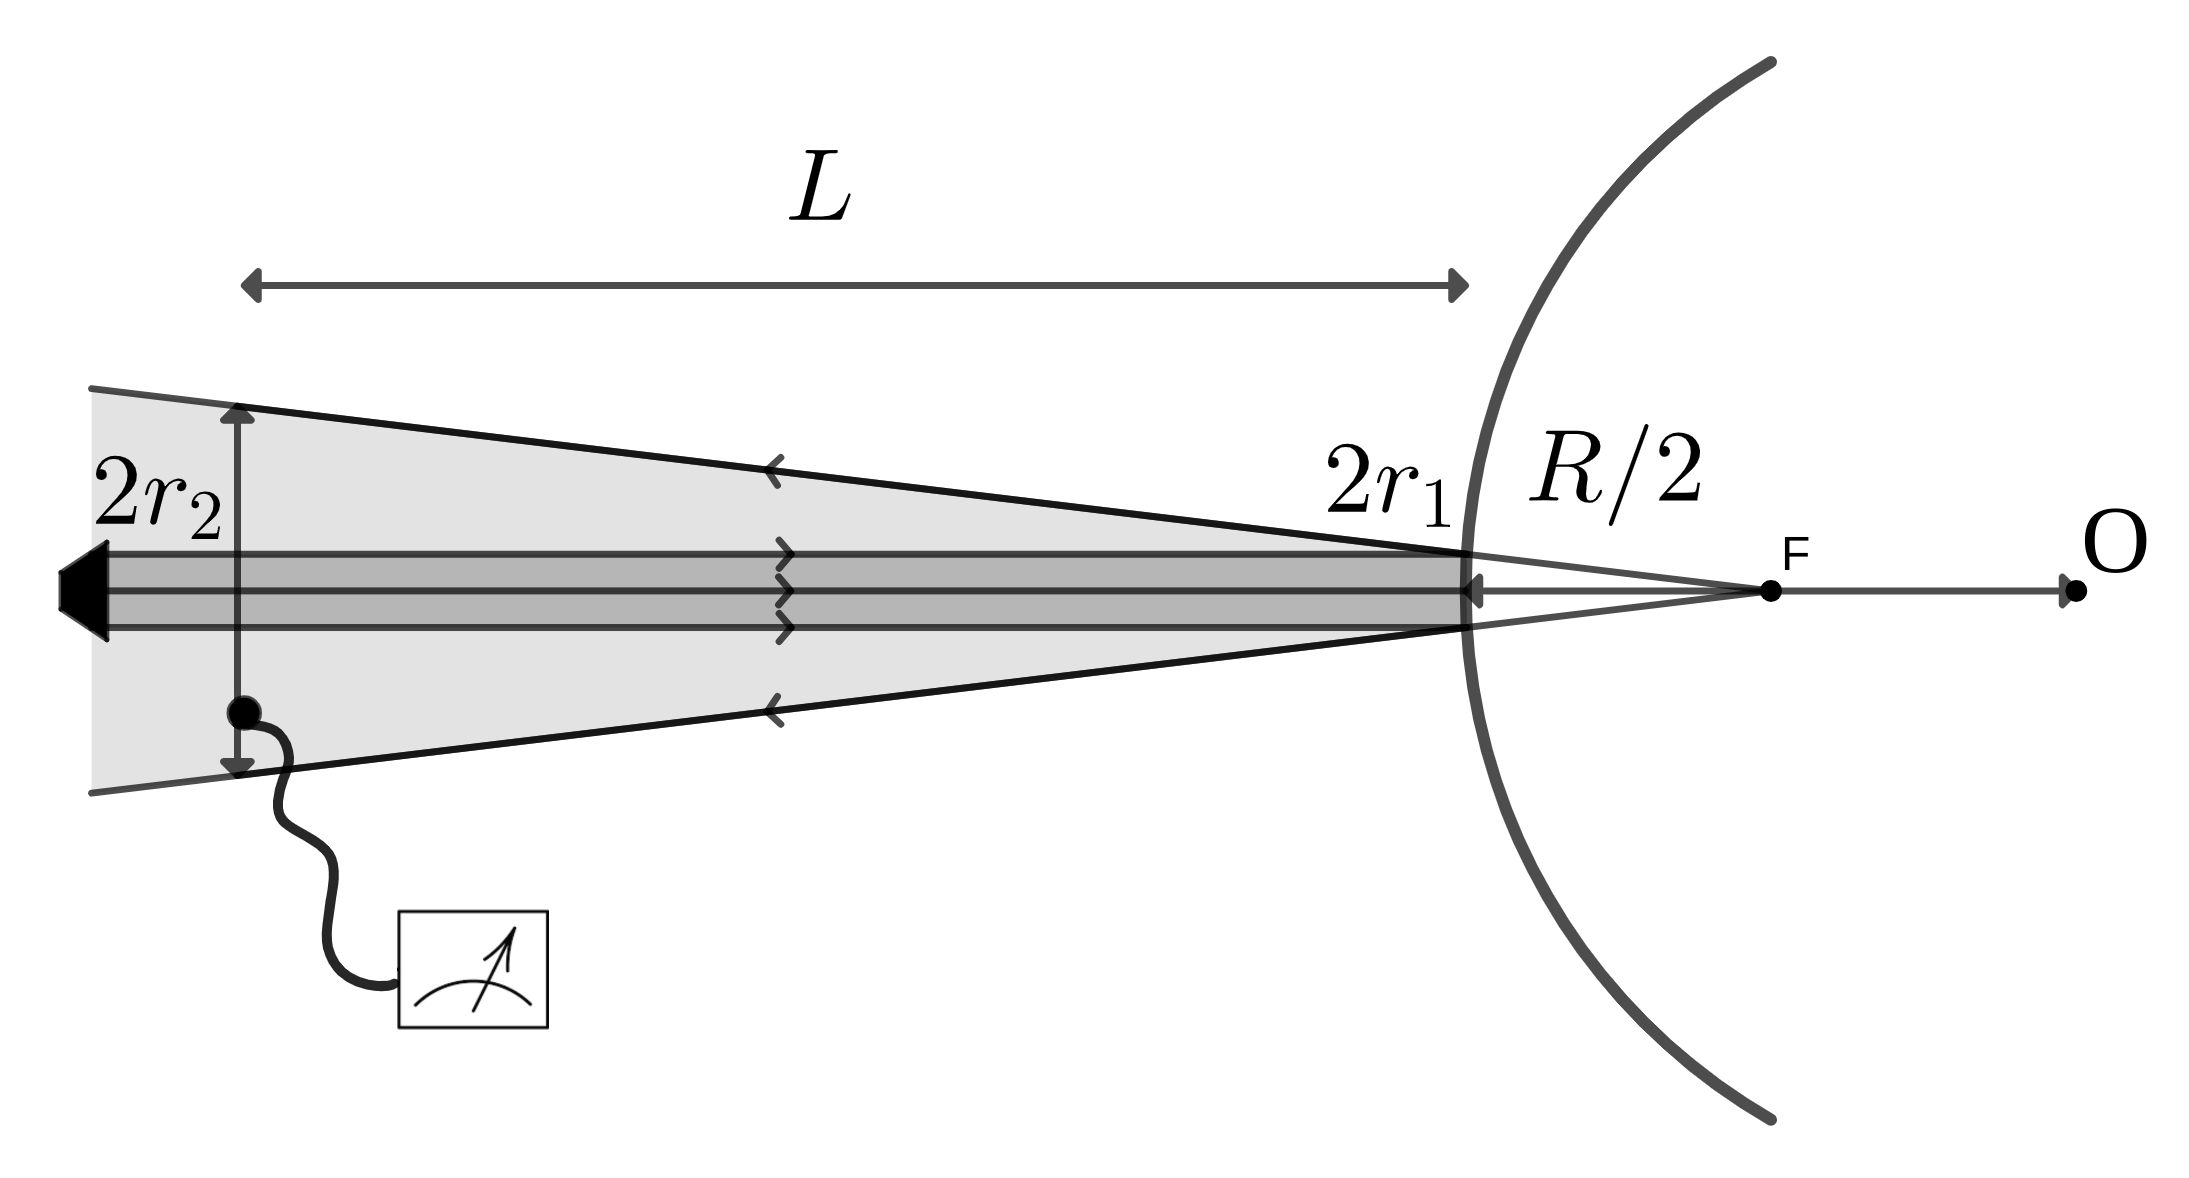
\includegraphics[width=0.6\linewidth]{Joonised/hajumine-lah.png}
\end{figure}

\yl{VALGUSDIOODID}
\punktid{8} \autor{Hans Daniel Kaimre}

Kuivõrd LEDide nominaalne voolutugevus on võrdne, on mõistlik need ühendada omavahel jadamisi, nii nagu Mari seda tegi. Pingelang üle LEDide normaaltingimustel on $U_1+U_2=\SI{3}{\V}+\SI{3.5}{\V}=\SI{6.5}{\V}$, mis on tunduvalt vähem kui patarei klemmipinge $U=\SI{12}{V}$. Järelikult tuleb vooluringi ühendada LEDidega jadamisi takisti, millel pingelang oleks $U_R=U-U_1-U_2=\SI{12}{\V}-\SI{6.5}{\V}=\SI{5.5}{\V}$. Takisti väärtuse saame leida lihtsalt Ohmi seadusest, kuna takistit läbiv voolutugevus peab olema võrdne LEDe läbiva voolutugevusega: $R=U_R/I_1=\SI{5.5}{\V}/\SI{30}{\milli\A}=\SI{183}{\ohm}$.

\begin{figure}[h]
    \centering
    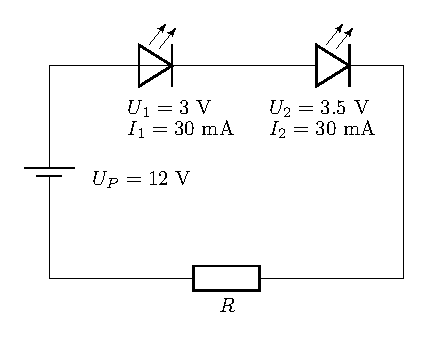
\includegraphics[width=0.5\linewidth]{Joonis_LEDid_lah.pdf}
\end{figure}


\yl{GALILEO TERMOMEETER}
\punktid{8} \autor{Jaan Kalda}

Olgu kuulikese koguruumala $V$; sellisel juhul vee tihedus 20 kraadi juures $\rho_1$ rahuldab tasakaalutingimust $\rho_1V=m_1$ \p{1}. Sarnase seose saame 22-kraadise kuulikese kogumassi jaoks, $m_2=\rho_2V$, kus  $\rho_2$ tähistab vee tihedust 22 kraadi juures \p{1}. Ühikmassi vee ruumala 20 kraadi juures on $V_1=1/\rho_1$ ja 22 kraadi juures ---  $V_2=1/\rho_2$ \p{1}. Teisest küljest $V_2=V_1(1+k\Delta T)$, kus $\Delta T=\SI 2\celsius$ \p{1}. Seetõttu $\rho_2=1/V_2=1/[V_1(1+k\Delta T)]=\rho_1/(1+k\Delta T)$ \p{1}. Et  esimese kahe valemi põhjal $m_2=\rho_2V=m_1\rho_2/\rho_1$ \p{1}, siis  $m_2=m_1/(1 + k\Delta T) $ \p{1}. Numbriliselt saame $m_2= \SI{19.9916}g$ \p{1}. 

\newpage
\yl{AMOKSITSILLIIN}
\punktid{8} \autor{Marten Rannut}

Arvutame Juku efektiivse doosi: $m_d = \SI{70}{\kilogram} \cdot \SI{140}{\micro\gram\per\kilogram} = \SI{9800}{\micro\gram} = \SI{9,8}{\milli\gram}$ \p{2}. Olgu $t_d$ aeg kahe tableti võtmise vahel. Me teame, et tablet tuleb võtta ajal, kui ravimi kontsentratsioon kehas langeb $m = \SI{500}{mg}$ pealt $m_d = \SI{9.8}{mg}$ peale. (Järgnevate tablettide puhul on algne kontsentratsioon natukene kõrgem, $\SI{509.8}{mg}$, sest lisandub eelmine minimaalne efektiivne doos, kuid erinevus on piisavalt väike, et see tühiseks lugeda.)

Kuna $t$ on poolestusaeg, siis järelikult $m_d = m(\frac 12)^{t_d/t}$ \p{3}, kust 
$\frac{t_d}{t} = \log_{1/2}(m_d/m)$, seega $t_d = \frac{\log(m_d/m)}{\log(1/2)}t$ \p{2}. Arvuliselt leiame $t_d = \frac{\log(9.8/500)}{\log(1/2)}\cdot \SI{1.4}{\hour} \approx \SI{7.94}{\hour} \approx \SI{8}{\hour}$ \p{1}.

(Kui logaritmi ei ole osatud võtta, aga on proovimise teel leitud, et vastus on $5t = \SI{7}{\hour}$ ja $6t=\SI{8.4}{\hour}$ vahel, siis \p{-2}, st ülesande eest kokku max \p{6}.)

\textit{Märkus:} Ülesanne on eluga päris kattuv, 500 mg amoksitsilliini 3x päevas on päris tavaline retsept.

\yl{MITTEELASTNE NÖÖR}
\punktid{10} \autor{Päivo Simson}

\begin{wrapfigure}{r}{0.5\textwidth}
  \vspace{-1em}
  \begin{center}
    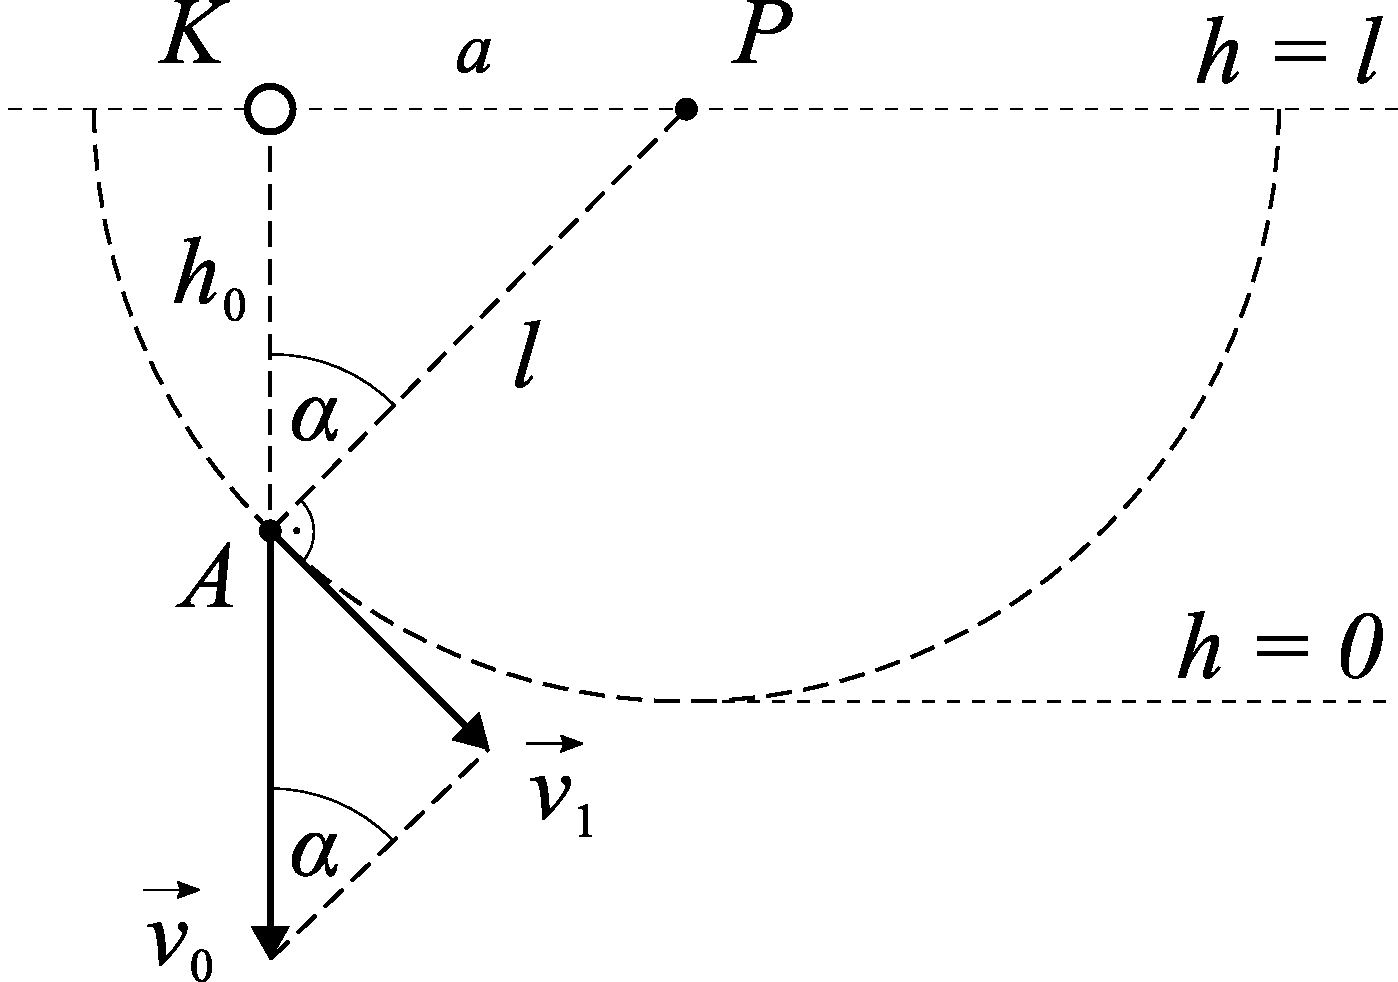
\includegraphics[width=1\linewidth]{mn_sol_1.pdf}
  \end{center}
  \vspace{-1em}
\end{wrapfigure}

Kuulike langeb kõigepealt vabalt kõrguse $h_0=\sqrt{l^2-a^2}$ võrra ja saavutab punktis $A$ kiiruse $v_0=\sqrt{2gh_0}$. Selleks hetkeks on nöör sirge ja toimub löök, mille korral tagasipõrget ei toimu, sest nöör on mitteelastne. Löögi käigus kaotab kuulike nöörisihilise kiiruse $\Vec{v}_0$ komponendi ja seega ka osa energiast (kaotatud energia läheb nöörile, mis selle arvelt soeneb). Kuulike jätkab liikumist mööda pikkusega $l$ määratud ringjoone kaart. Säilib ainult kiiruse komponent $v_1$, mis on paralleelne ringjoone puutujaga punktis A: $v_1=v_0\sin\alpha=v_0a/l=\sqrt{2gh_0}\,a/l$. Seega on kuulikese koguenergia vahetult pärast punkti A jõudmist
\[E = \frac{mv_1^2}{2}+mg(l-h_0)=mgh_0\frac{a^2}{l^2}+mg(l-h_0)=\]
\[=mgl\left(1-\frac{h_0}{l}\left(1-\frac{a^2}{l^2}\right)\right)=mgl\left(1-\left(1-\frac{a^2}{l^2}\right)^{\frac{3}{2}}\right).\]
Vabalangemisele järgnevalt jääb kuulike mööda ringjoone kaart võnkuma. Trajektoori kõrgeimas punktis on kuulikese kiirus null ja koguenergia on järelikult $E=mgH$, kus $H$ on otsitav maksimaalne kõrgus. Võrdsustades koguenergia avaldised saame
\[H=l\left(1-\left(1-\frac{a^2}{l^2}\right)^{\frac{3}{2}}\right).\]

\begin{wrapfigure}{r}{0.5\textwidth}
\vspace{-1cm}
  \begin{center}
    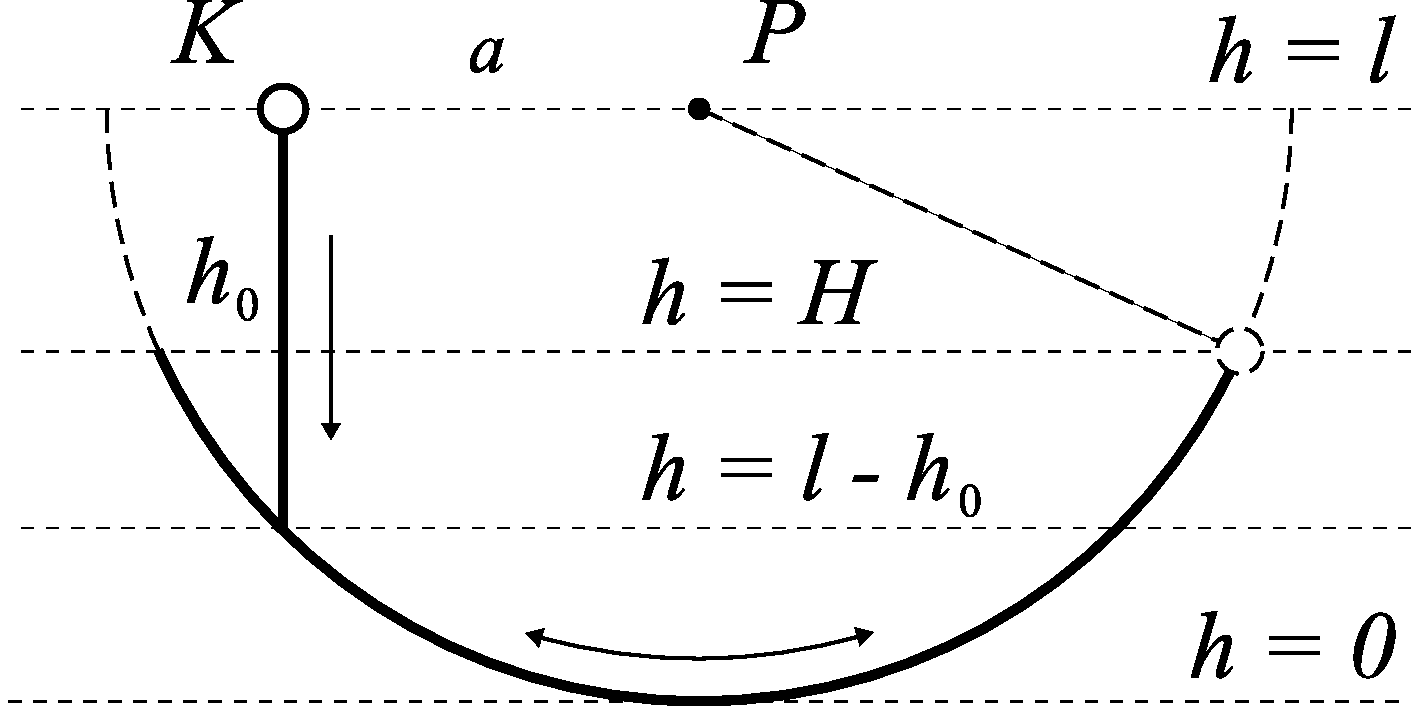
\includegraphics[width=1\linewidth]{mn_sol_2.pdf}
  \end{center}
  \vspace{-1.0cm}
\end{wrapfigure}

Trajektoori joonestamiseks võrdleme kõrgusi $H$ ja $l-h_0$. Et $1-a^2/l^2=h_0^2/l^2$ ja $h_0/l<1$, siis
$l(1-h_0^3/l^3)>l(1-h_0/l)$
ehk $H>l-h_0$.
Kuuli trajektoor on näidatud parempoolsel joonisel paksu pideva joonega. Võrratuse $H>l-h_0$ näitamiseks piisab ka tähelepanekust, et punktis $A$, pärast löögi toimumist, on pallil endiselt kineetiline energia olemas ja seega ei saa punkt $A$ olla edasise liikumise kõrgeim punkt.


\yl{PALGID VEES}
\punktid{10} \autor{Jaan Kalda}

Süsteemile vesi+palgid mõjub raskusjõud, mille tasakaalustab jõud $pS-2T$, kus $T$ on jõud, millega niit tõmbab kumbagi palki. Idee vaadelda süsteemi vesi+palgid koos annab \p{2}; tasakaalutingimusest saadud raskusjõu avaldis $pS-2T$ annab \p{2}. Väiksema palgi tasakaalutingimusest saame, et $T=(\rho_v- \rho)Vg$ \p{1}. Kui niit katki lõigata, siis niidi pinge kaob, kuid süsteemile vesi+palgid mõjub raskusjõud jõud peab samaks jääma \p{1}. Seega rõhumisjõu muutus $S\Delta p=2T$ \p{1}. Et $\Delta p=\rho_vg\Delta h$ \p{1}, siis veetase langeb kõrguse $\delta h=2T/\rho_vgS=2(\rho_v- \rho)V/\rho_vS=\SI{2.4}{\cm}$ (valem \p{1}, arvväärtus \p{1}).

Alternatiivne lahendus.  Väiksema palgi tasakaalutingimusest saame, et $T=(\rho_v- \rho)Vg$ \p{1}. Olgu suurema palgi koguruumala $U$, millest vee all on ruumala $W$. Sellisel juhul saame selle tasakaalutingimuseks $\rho_v Wg= \rho Ug+T$ \p{1}. Kahest avaldisest saame kokku $W=kU+V-kV$ \p{1}, kus $k=\rho/\rho_v$. Kui nöör on katki, siis on palkide veealuste osade ruumalad tasakaalutingimusest tulenevalt vastavalt $Vk$ ja $Uk$ (\p{1+1}). Enne oli palkide veealuste osade ruumalade summa $W+V$ \p{1} ja pärast --- $Vk+Uk$ \p{1}, seega veealuste osade ruumala vähenes $W+V-Vk-Uk=2V(1-k)$ võrra \p{1}, mistõttu alanes veetase $2V(1-k)/S=\SI{2.4}{\cm}$ võrra (valem \p{1}, arvväärtus \p{1}).

\yl{HERMEETILINE SAUN}
\punktid{12} \autor{Hannes Kuslap}

Kuna enne kütma hakkamist oli saunauks lahti, siis järelikult olid rõhud saunas ja saunast väljas tasakaalustunud; seega kui $T=T_1$, oli õhurõhk saunas $p_0$ \p{1}. Kütmise ajal oli saunauks kinni ja saun hermeetiline, seega õhu ruumala saunas oli konstantne \p{1}. Ideaalgaasi võrrandist $pV=nRT$ \p{1} leiame seega, et $p \propto T$, see tähendab $\frac{p_2}{p_1} = \frac{T_2}{T_1}$. Järelikult õhurõhk saunas pärast kütmist on $p_2 = \frac{T_2}{T_1}p_0$ \p{1}. (Alternatiivselt võib välja arvutada ruumala $V$ ning leida $nR$ väärtus ja selle abil arvutada $T_2$.) Rõhkude vahe tõttu avaldub uksele summaarne jõud $F_{\rm õhk} = (p_2-p_0)hl$ \p{1}. Aivo maksimaalne lükkejõud on aga piiratud tema jalgade hõõrdejõu poolt $F_{\rm lüke} = \mu m g$ (suurema jõu korral hakkaksid Aivo jalad libisema) \p{1}. Eeldades, et õhurõhk mõjub uksele ühtlaselt, siis keskmine rõhujõu õlg on $L_{\rm õhk} = \frac{l}{2}$. Ukselink asub aga servas, nii et lükkejõu õlg on $L_{\rm lüke} = l$. Kangi reegli abil uksehinge suhtes leiame, et uks avaneb, kui $F_{\rm lüke}L_{\rm lüke} > F_{\rm õhk}L_{\rm õhk}$, see tähendab $2F_{\rm lüke} > F_{\rm õhk}$ \p{2} (kui kordaja 2 puudu, siis \p{0}). Seega ukse avanemise tingimus on $2\mu m g > \left(\frac{T_2}{T_1}-1\right)p_0hl$ \p{1}. Vasaku poole arvuline väärtus on $2\cdot\num{0.6}\cdot \SI{100}{kg} \cdot \SI{9.8}{\N\per\kg} \approx \SI{1180}{N}$ \p{1}. Teades, et $T_1 = 273+\SI{20}{K} = \SI{293}{K}$ ja $T_2 = 100+\SI{273}{K}=\SI{373}{K}$, leiame, et parema poole väärtus on $\left(\frac{\SI{373}{K}}{\SI{293}{K}}-1\right)\cdot \SI{101000}{Pa} \cdot \SI{1.8}{m}\cdot\SI{0.8}{m}\approx \SI{39700}{N}$ \p{1}. Kuna $\SI{39700}{N} > \SI{1180}{N}$, siis Aivo ei saa ust lahti (õige järelduse eest \p{1} ainult siis, kui lahendus on füüsikaliselt korrektne).

\yl{LAETUD KUUL}
\punktid{12} \autor{Konstantin Dukatš}

Alguses on kuuli laeng väike, nii et pinge ja seega ka vool takistil $R$ on väike. Seetõttu on elektronidelt saabuv laengu vool suurem kui väljavoolav vool. Seetõttu kuhjub laeng kuuli pinnale kuni voolude tasakaalustamiseni.

Olgu $S=\pi a^2$ kuuli ristlõike pindala. Saame kirjutada voolu tasakaalu võrrandi:
$$I = \frac{\Delta Q}{\Delta t} = -e \frac{\Delta N}{\Delta t} = -e n_e v S = -e n_e v \pi a^2.$$
Pinge takistil on võrdne $V = I R = \varphi - 0 = \varphi$, kus $\varphi$ on potentsiaal kuuli pinnal, 0 on maapinna potentsiaal.
$$\varphi = -e n_e v \pi a^2 R,$$
$$\varphi = \frac{1}{4 \pi \varepsilon_0} \frac{Q}{a}.$$
Siit leiame:
$$Q = 4 \pi \varepsilon_0 \varphi a = -4 \pi^2 \varepsilon_0 e n_e v a^3 R.$$
Eeldus, et $v \gg n_e e^2 a^2 R / m$, oli vajalik selleks, et ignoreerida, et laetud kuul on elektronide liikumisele vastu, tõrjudes neid.


\yl{PÕRKED}
\punktid{14} \autor{Päivo Simson}

\begin{wrapfigure}{r}{0.4\textwidth}
\vspace{-1.1cm}
  \begin{center}
    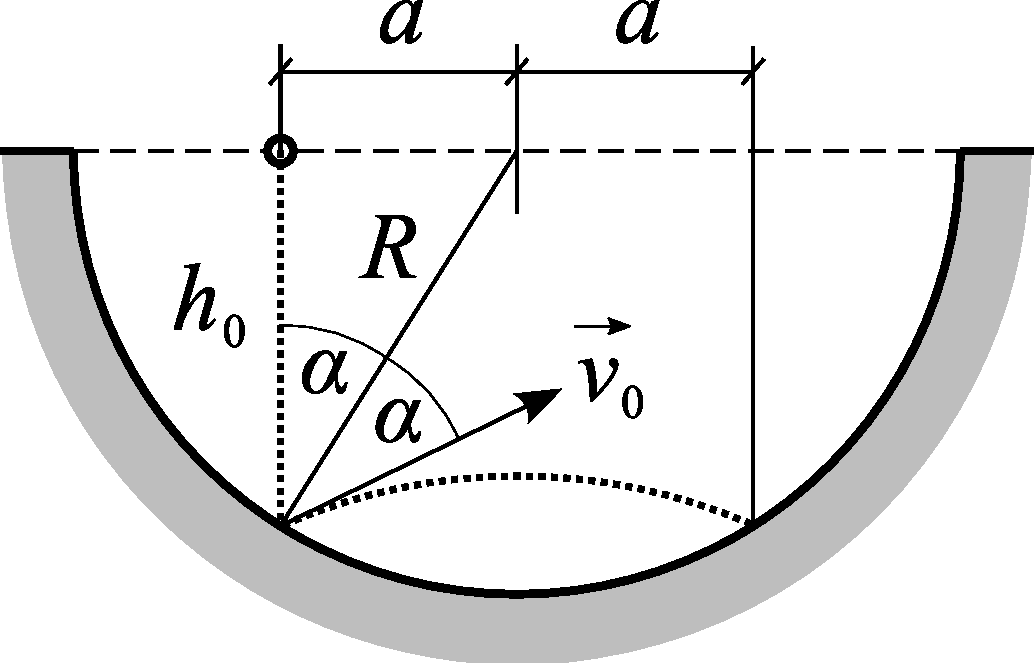
\includegraphics[width=1\linewidth]{porked_sol.pdf}
  \end{center}
  \vspace{-1cm}
\end{wrapfigure}

\textbf{Lahendus 1}

Ilmselt on lihtsaim perioodiline liikumine selline, mille korral kummipall jääb põrkuma kahe punkti vahel, mis mõlemad on kera keskteljest kaugusel $a$ \p{1}. Uurime, kas selline lahend on võimalik, ja kui on, siis milline peab olema kaugus $a$. 

Kuni esimese põrkeni langeb pall vabalt kõrguse $h_0=\sqrt{R^2-a^2}$ võrra ja saavutab kiiruse $v_0=\sqrt{2gh_0}$ \p{1}. Elastne põrge toimub nurga $2\alpha$ all \p{1} ja edasi liigub pall mööda parabooli, mille haripunkt asub poolkera teljel \p{1}. Paraboolil liikudes on algkkiiruseks $\vec v_0$, mis on horisondi suhtes nurga $90^\circ-2\alpha$ all \p{1}. Kiiruse komponentide ajaline sõltuvus kahe põrke vahelisel ajal on
\begin{align*}
    &v_x=v_0\cos(90^\circ-2\alpha)=v_0\sin 2\alpha=const, \qquad\p{1}\\
    &v_y=v_0\sin(90^\circ-2\alpha)-gt=v_0\cos 2\alpha-gt. \qquad\p{1}
%    &x=v_{x}t=v_0t\sin 2\alpha\\
%    &y=v_{0y}t-gt^2/2
\end{align*}
Kui koordinaatide alguseks valida põrkekoht, siis on parabooli haripunktis $x=v_xt_h=a$, kus $t_h$ on haripunkti jõudmiseks kuluv aeg \p{1}. Lisaks on haripunktis $v_y=0$, millest saame
$t_h=v_0\cos 2\alpha/g$ \p{1}. Võrdus $a=v_xt_h$ annab nüüd
\[a=\frac{v_0^2\sin2\alpha\cos 2\alpha}{g}=2h_0\sin2\alpha\cos 2\alpha\qquad \p{1}\]
Jagame selle võrduse $h_0$-ga ja teisendame saadava võrduse paremat ja vasakut poolt:
\begin{align*}
a/h_0&=2\sin2\alpha\cos 2\alpha\\
\tan\alpha&=4\sin\alpha\cos\alpha(\cos^2\alpha-\sin^2\alpha)\\
\sin\alpha/\cos\alpha&=4\sin\alpha\cos\alpha(1-2\sin^2\alpha)\qquad \p{1}\\
\end{align*}
Saime võrrandi nurga $\alpha$ leidmiseks. Et $\alpha=0$ vastab juhule $a=0$, siis see lahend meile ei sobi. Korrutades viimast võrdust koosinusega ja jagades siinusega saame
\[1=4\cos^2\alpha(1-2\sin^2\alpha)=4(1-\sin^2\alpha)(1-2\sin^2\alpha)\]
Tähistame $x=\sin\alpha$, viime liikmed ühele poole võrdusmärki ja litsustame.
\[4(1-x^2)(1-2x^2)-1=0,\]
\[8x^4-12x^2+3=0.\qquad \p{2}\]
Saime ruutvõrrandi $x^2$ suhtes, mille lahend on
\[x^2=\frac{12\pm\sqrt{12^2-4\cdot8\cdot3}}{16}=\frac{12\pm\sqrt{48}}{16}=\frac{3\pm\sqrt{3}}{4}.\]
Plussiga lahend ei sobi, sest $\sin\alpha$ ei saa olla ühest suurem. Järelikult
\[x=\sin\alpha=\frac{\sqrt{3-\sqrt{3}}}{2},\]
ehk
\[a=R\frac{\sqrt{3-\sqrt{3}}}{2}\approx\num{0.563}R.\qquad \p{1}\]
Näeme, et kahe punkti vahel põrkuv liikumine on võimalik ja see realiseerub ülaltoodud $a$ väärtuse korral. Täpsemalt liigub pall ülevalt alla, siis mööda parabooli paremale, siis vertikaalselt üles ja alla, siis mööda parabooli tagasi esimese põrke punkti, uuesti üles ja alla jne.

\textbf{Lahendus 2}

Eeldame, et lihtsaim perioodiline liikumine on selline, mille korral kummipall jääb põrkuma kahe punkti vahel, mis mõlemad on kera keskteljest kaugusel $a$ \p{1}. Kuni esimese põrkeni langeb pall vabalt kõrguse $h_0$ võrra. Elastne põrge toimub nurga $2\alpha$ all \p{1} ja edasi liigub pall mööda parabooli, mille haripunkt asub eelduse põhjal poolkera teljel \p{1}.

\begin{wrapfigure}{r}{0.6\textwidth}
\vspace{-1.1cm}
  \begin{center}
    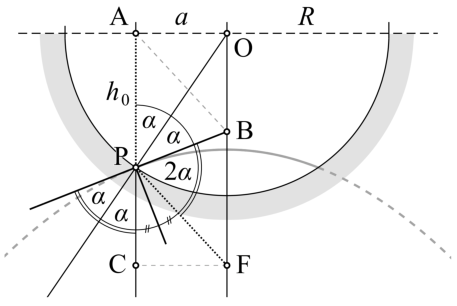
\includegraphics[width=1\linewidth]{porked-sol2.png}
  \end{center}
  \vspace{-0.5cm}
\end{wrapfigure}

Parabooli omadustest on teada, et vertikaalne kiir $CP$ peegeldub parabooli fookusesse $F$ \p{2}. Et langemisnurk ja peegeldumisnurk on võrdsed \p{1}, siis järelikult $\angle{FPB}=2\alpha$ \p{1}. Kolmnurgad $PAB$ ja $PBF$ on sarnased, järelikult lõik $PF=h_0$ \p{1} (seega on punkti $O$ läbiv horisontaaljoon parabooli juhtjooneks). Kolmnurgast $POA$ saame
\[\frac{a}{h_0}=\tan\alpha\qquad \p{1}\]
ja kolmnurgast $PCF$
\[\frac{a}{h_0}=\sin(180^\circ-4\alpha)=\sin(4\alpha). \qquad \p{1}\]
Tulemuseks on võrrand $\tan\alpha=\sin 4\alpha$, ehk
\[\frac{\sin\alpha}{\cos\alpha}=4\sin\alpha\cos\alpha(1-2\sin^2\alpha), \qquad \p{1}\]
mille lahendamisel saame (vt lahendus 1)
\[\sin\alpha=\frac{\sqrt{3-\sqrt{3}}}{2}=\frac{a}{R}. \qquad \p{3}\]


\end{document}